\begin{frame}{}

\noindent\makebox[\linewidth][c]{%
\begin{minipage}{\linewidth}

  \begin{minipage}{0.45\linewidth}
    \scriptsize
    \begin{figure}
      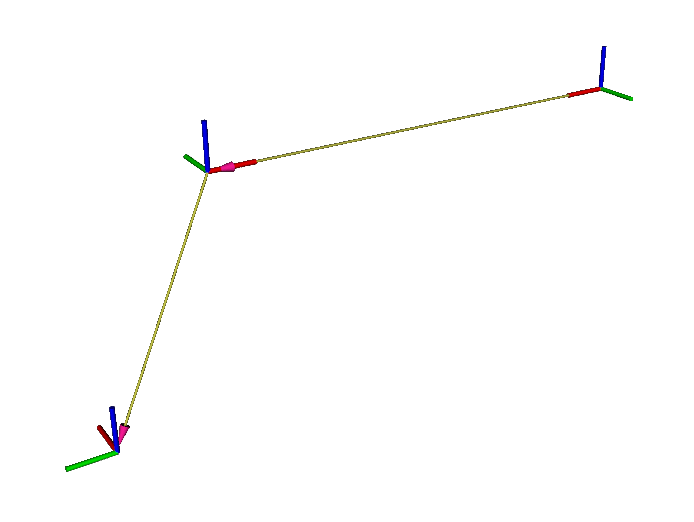
\includegraphics[height=120pt,width=159.54pt]{./figures/slides/ch3/antenna_frame}
      \vspace{1cm}
      \caption{Συστήματα αναφοράς ρομπότ, κεραίας, και τυχαίου προϊόντος}
      \begin{textblock}{4}(0.8,8.3)
        \texttt{base\_footprint}
      \end{textblock}
      \begin{textblock}{4}(1.8,4.2)
        \texttt{antenna\_frame}
      \end{textblock}
      \begin{textblock}{4}(4.5,3.3)
        \texttt{product\_n\_frame}
      \end{textblock}
    \end{figure}
  \end{minipage}
  \hspace{0.1cm}
  \begin{minipage}{0.45\linewidth}\vspace{2cm}
    \begin{figure}\centering
      \scalebox{0.5}{

\tikzset{every picture/.style={line width=0.75pt}} %set default line width to 0.75pt

\begin{tikzpicture}[x=0.75pt,y=0.75pt,yscale=-1,xscale=1]
%uncomment if require: \path (0,300); %set diagram left start at 0, and has height of 300
\path(100,100);

%Straight Lines [id:da535044070379217]
\draw    (154.3,52) -- (154.3,80) ;
\draw [shift={(154.3,82)}, rotate = 270] [color={rgb, 255:red, 0; green, 0; blue, 0 }  ][line width=0.75]    (10.93,-3.29) .. controls (6.95,-1.4) and (3.31,-0.3) .. (0,0) .. controls (3.31,0.3) and (6.95,1.4) .. (10.93,3.29)   ;
%Straight Lines [id:da03696969507445824]
\draw    (153.3,111) -- (153.3,139) ;
\draw [shift={(153.3,141)}, rotate = 270] [color={rgb, 255:red, 0; green, 0; blue, 0 }  ][line width=0.75]    (10.93,-3.29) .. controls (6.95,-1.4) and (3.31,-0.3) .. (0,0) .. controls (3.31,0.3) and (6.95,1.4) .. (10.93,3.29)   ;
%Straight Lines [id:da46122910611053514]
\draw    (462.3,56) -- (462.3,145) ;
\draw [shift={(462.3,54)}, rotate = 90] [color={rgb, 255:red, 0; green, 0; blue, 0 }  ][line width=0.75]    (10.93,-3.29) .. controls (6.95,-1.4) and (3.31,-0.3) .. (0,0) .. controls (3.31,0.3) and (6.95,1.4) .. (10.93,3.29)   ;
%Right Arrow [id:dp5085649971129671]
\draw   (257,147) -- (299,147) -- (299,137) -- (327,157) -- (299,177) -- (299,167) -- (257,167) -- cycle ;

% Text Node
\draw    (60.94,27) -- (249.94,27) -- (249.94,52) -- (60.94,52) -- cycle  ;
\draw (155.44,39.5) node   [align=left] {Εκτίμηση θέσης προϊόντων};
% Text Node
\draw    (64.05,86) -- (244.05,86) -- (244.05,111) -- (64.05,111) -- cycle  ;
\draw (154.05,98.5) node   [align=left] {Εκτίμηση στάσης κεραιών};
% Text Node
\draw    (65.04,145) -- (241.04,145) -- (241.04,170) -- (65.04,170) -- cycle  ;
\draw (153.04,157.5) node   [align=left] {Εκτίμηση στάσης ρομπότ};
% Text Node
\draw    (344.21,145) -- (581.21,145) -- (581.21,170) -- (344.21,170) -- cycle  ;
\draw (462.71,157.5) node   [align=left] {Σφάλμα εκτίμησης στάσης ρομπότ};
% Text Node
\draw    (334.03,25) -- (592.03,25) -- (592.03,50) -- (334.03,50) -- cycle  ;
\draw (463.03,37.5) node   [align=left] {Σφάλμα εκτίμησης στάσης προϊόντων};


\end{tikzpicture}

}
      \vspace{0.8cm}
      \caption{Η εκτίμηση της θέσης των προϊόντων εξαρτάται από το σφάλμα της
               εκτίμησης της στάσης του ρομπότ}
    \end{figure}
  \end{minipage}
\end{minipage}
}


\end{frame}
